\documentclass[12pt,a4paper]{report}

% --- Paquetes de Idioma y Codificación ---
\usepackage[utf8]{inputenc}
\usepackage[T1]{fontenc}
\usepackage[spanish, es-tabla]{babel}

% --- Diseño de Página ---
\usepackage{geometry}
\geometry{top=2.5cm, bottom=2.5cm, left=3cm, right=3cm}

% --- Matemáticas y Símbolos ---
\usepackage{amsmath, amssymb, amsthm}

% --- Colores y Cajas ---
\usepackage[dvipsnames]{xcolor}
\usepackage[most]{tcolorbox}

% Caption

\usepackage{caption}

% Gráficos

\usepackage{graphicx}

% Espaciadora

\newcommand{\esp}{\vspace{0.5cm}}

% promedio

\newcommand{\prom}[1]{\left\langle #1 \right\rangle}

% ket

\newcommand{\ket}[1]{| #1 \rangle}

% bra

\newcommand{\bra}[1]{\langle #1 |}

% braket

\newcommand{\braket}[2]{\langle #1 | #2 \rangle}

% Bibliografía

\usepackage[style=apa, backend=biber]{biblatex} % Estilo APA
\addbibresource{biblio.bib} % Nombre de tu archivo .bib

% Configuración de cajas personalizadas
\newtcolorbox{importante}{
	colback=red!5!white,
	colframe=red!75!black,
	title=Importante,
	fonttitle=\bfseries
}

\newtcolorbox{nota}{
	colback=blue!5!white,
	colframe=blue!75!black,
	title=Nota,
	fonttitle=\bfseries
}

% Definición de la caja de bibliografía
\newtcolorbox{bibliografia}{
	colback=gray!5!white,
	colframe=gray!75!black,
	title=Bibliografías útiles,
	fonttitle=\bfseries,
	breakable
}

% Socrative para óptica 2

\newtcolorbox{Socrative}{
	colback=orange!5!white,
	colframe=orange!75!black,
	title=Socrative,
	fonttitle=\bfseries,
	breakable
}

% Float

\usepackage{float}

% --- Hipervínculos ---
\usepackage{hyperref}
\hypersetup{
	colorlinks=true,
	linkcolor=blue,
	filecolor=magenta,      
	urlcolor=cyan,
}

% --- Datos del Documento ---
\title{Óptica II}
\author{Chengyu Jin}
\date{\today}

\begin{document}
	
	\maketitle
	
	\tableofcontents
	\newpage
	
	\chapter{Teoría difraccional de la formación de imagen}
	
	\section{Introducción}
	
	\begin{figure}[H]
		\centering
		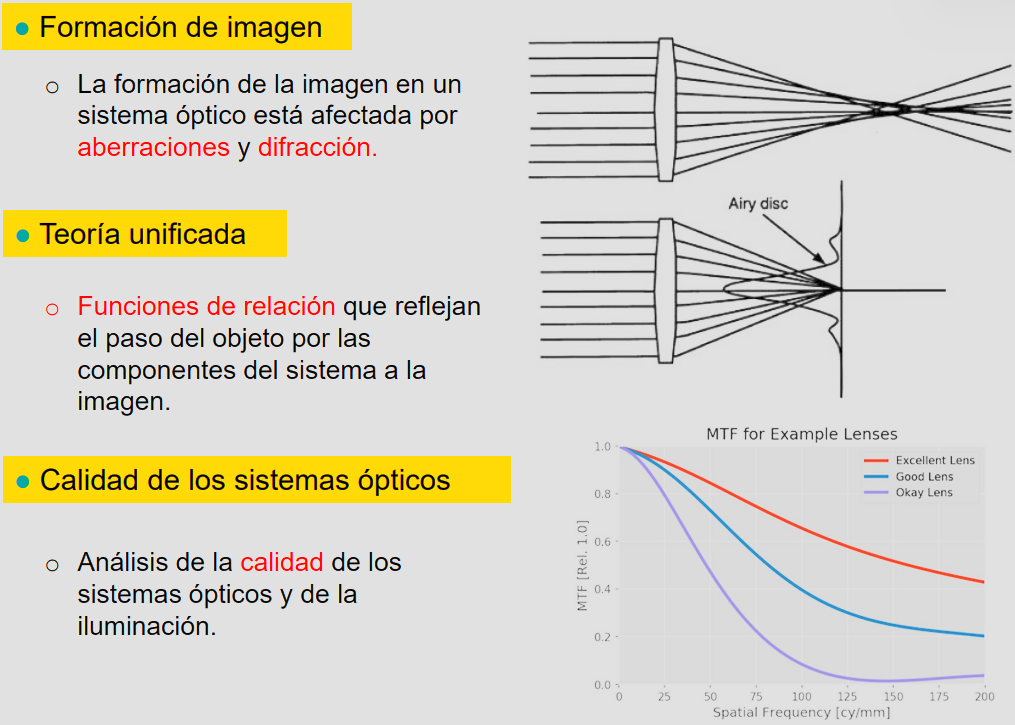
\includegraphics[width=0.7\textwidth]{IMG/intro.png}
	\end{figure}
	
	\esp
	
	Vamos a abordar en este tema el estudio de la formación de imágenes aplicando el formalismo de la difracción. A diferencia de lo estudiado en Óptica Geométrica, donde el estudio de la formación de la imagen, incluso para el caso real de instrumentos aberrantes, se hacía suponiendo la propagación rectilínea de la luz, consideraremos ahora también el carácter ondulatorio de la misma. El proceso de formación de la imagen óptica es importante pues puede ayudar a un observador a obtener información visual más detallada de un objeto o bien proporcionar un registro permanente del objeto de interés. En cualquiera de los casos, será fundamental que la imagen de dicho objeto sea de calidad y similar al propio objeto, es decir, que la imagen que el sistema óptico proporciona del objeto mantenga una relación de semejanza con éste. Ahora bien, para la completa comprensión del proceso de formación de imágenes es necesario, por un lado, conocer las leyes que gobiernan el paso de la luz a través de todo sistema óptico, evaluando los efectos que dicho sistema pueda tener por la limitación física de su tamaño, y, por otro lado, es necesario conocer qué luz emite o refleja el objeto de interés y, lo que puede resultar más interesante, evaluar las propiedades de dicha luz respecto de su mayor o menor grado de coherencia. Debido a las dimensiones finitas de las aberturas de los instrumentos, el frente de onda es interceptado, poniéndose de manifiesto el fenómeno de la difracción, que no puede ser explicado con el modelo geométrico de propagación rectilínea de la luz. Tanto los fenómenos de la difracción como las aberraciones intervendrán por tanto conjuntamente en la calidad de la imagen y habrán de tenerse en cuenta para realizar un estudio completo de la formación de la imagen óptica y de la calidad de los instrumentos. La introducción del análisis de Fourier así como del formalismo de la teoría de la coherencia parcial de la luz serán, en gran parte, responsables de la realización de este estudio.
	
	\section{Formación de la imagen óptica}
	
	\subsection{PSF de un sistema óptico}
	
	\begin{figure}[H]
		\centering
		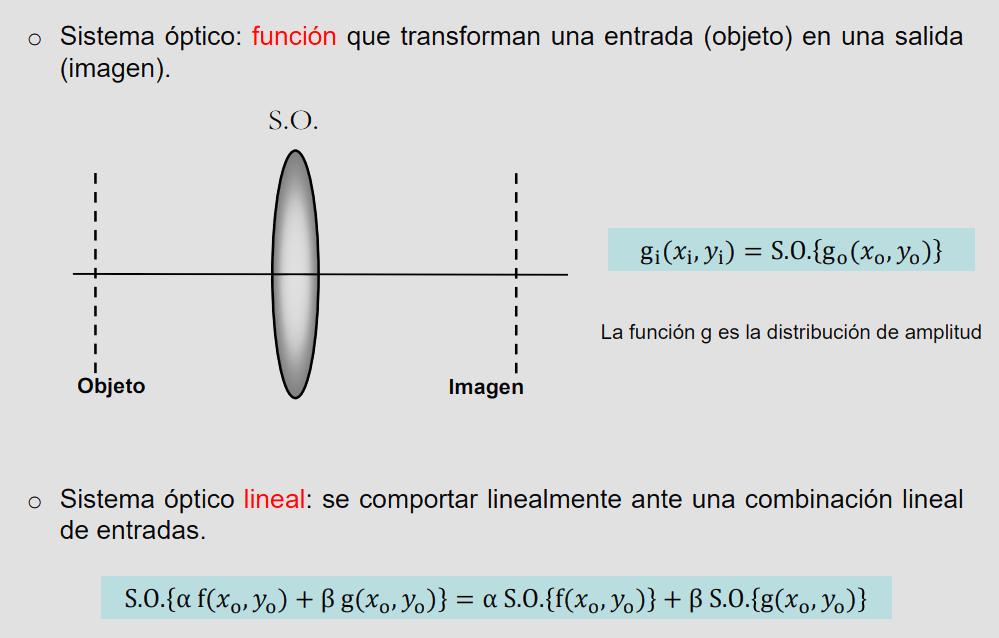
\includegraphics[width=0.7\textwidth]{IMG/sisopt.png}
	\end{figure}
	
	\esp
	
	Como hemos señalado en la sección anterior, vamos a considerar al sistema óptico como una función que transforma una distribución de amplitudes de entrada (el objeto) en otra distribución de amplitudes de salida (la imagen). Por simplicidad, consideraremos las dos distribuciones de amplitud como bidimensionales (objeto e imagen planos). La imagen la denotamos por $g_i(x_i, y_i)$ y el objeto por $g_o(x_o, y_o)$. Suponemos en el marco teórico que vamos a desarrollar que trabajamos con sistemas ópticos lineales. Es decir, que si el objeto es una combinación lineal de dos entradas al sistema, entonces la imagen se podrá calcular como una combinación lineal de las imágenes de cada elemento de la combinación objeto, con sus mismos pesos. Esta propiedad es fundamental para sentar las bases de la teoría difraccional de la formación de imagen y de la óptica de Fourier. La función transformadora será la función $S.O$
	
	\esp
	
	\begin{figure}[H]
		\centering
		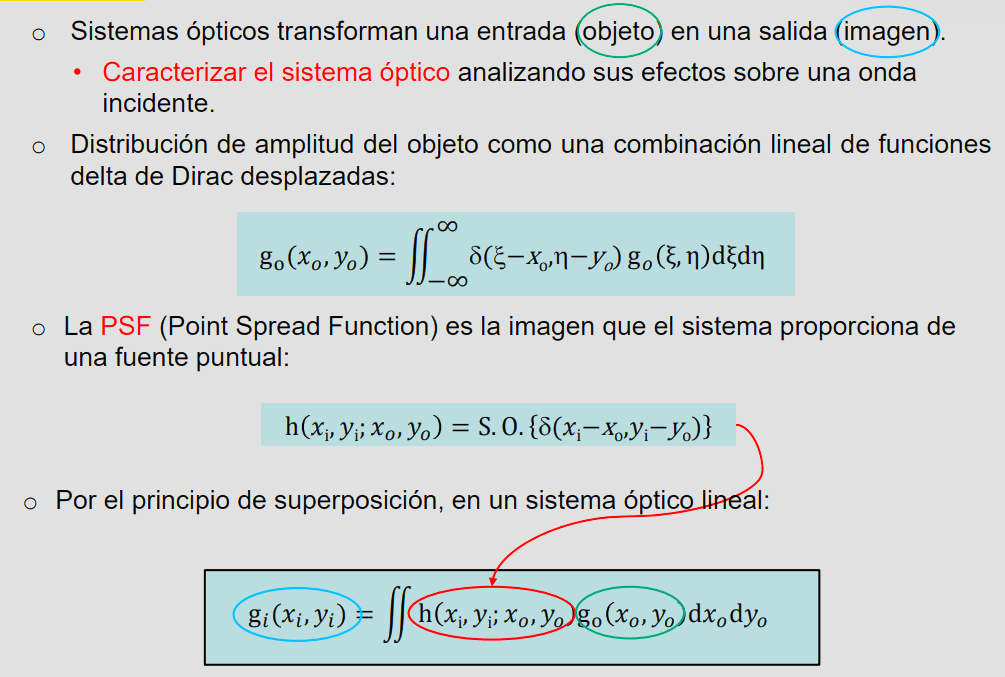
\includegraphics[width=0.7\textwidth]{IMG/sisopt2.png}
	\end{figure}
	
	\esp
	
	Utilizando las propiedades de la función delta de Dirac, podemos expresar el objeto como una combinación lineal de funciones delta desplazadas, con la propia distribución de intensidad del objeto como pesos en la combinación lineal. Por tanto, cuando transformamos el objeto mediante $S.O$, podemos aplicar que es una función lineal, y obtener la imagen como una integral doble de la función $g_o(\xi, \eta)$ multiplicada por $S.O(\delta(\xi - x_o, \eta - y_o))$. A la función $S.O$ llamamos Respuesta impulso del sistema óptico o también (porque sería algo parecido a calcular la imagen de un punto centrado en las coordenadas $(x_o, y_o)$), \textit{Point Spread Function} o PSF. 
	
	\esp
	
	\begin{figure}[H]
		\centering
		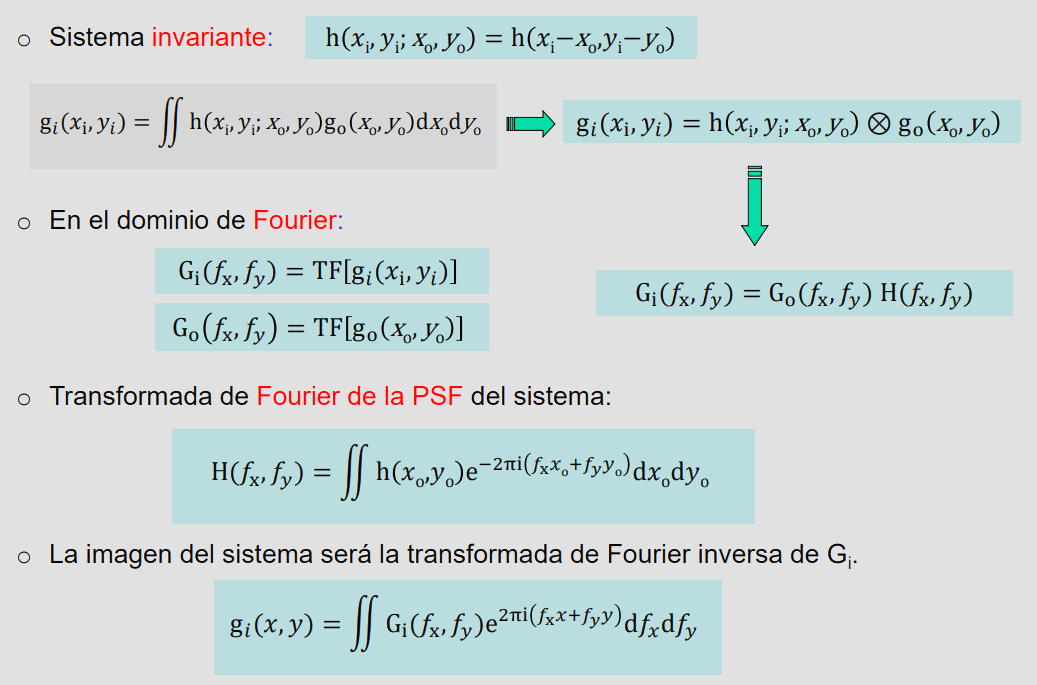
\includegraphics[width=0.7\textwidth]{IMG/sisopt3.png}
	\end{figure}
	
	\esp
	
	Si un sistema óptico verifica que su PSF es función sólo de las diferencias de coordenadas o desplazamientos (o sea, $h(x_i, y_i, x_0, y_0) = h(x_i - x_o, y_i - y_o)$), el sistema óptico se denomina invariante. Los sistemas ópticos invariantes tienen gran interés porque para ellos se verifica que la imagen es la convolución del objeto con la respuesta impulso del sistema. Esto es interesante porque permite utilizar las propiedades de la transformada de Fourier para poder calcular de forma más simple la distribución imagen. 
	
	\esp
	
	Recordemos que la Transformada de Fourier de una \textbf{convolución} de dos funciones es el producto de las Transformadas de Fourier de cada una de las dos funciones. Entonces,
	
	\begin{equation}
		G_i(f_x, f_y) = H(f_x, f_y)G_o(f_x, f_y).
	\end{equation}
	
	\esp
	
	Conociendo la Transformada de Fourier de la función respuesta impulso del sistema óptico ($H$) podemos entonces calcular $G_i$ de forma relativamente fácil, y, siempre que la imagen sea continua, podríamos pasar al espacio de coordenadas regular aplicando la Transformada de Fourier inversa, y determinar la distribución de intensidad en la imagen. En el siguiente apartado, vamos a aplicar este formalismo al caso de un sistema óptico simple como es la lente delgada.
	
	\subsection{La lente delgada como transformadora de fase}
	
	\begin{figure}[H]
		\centering
		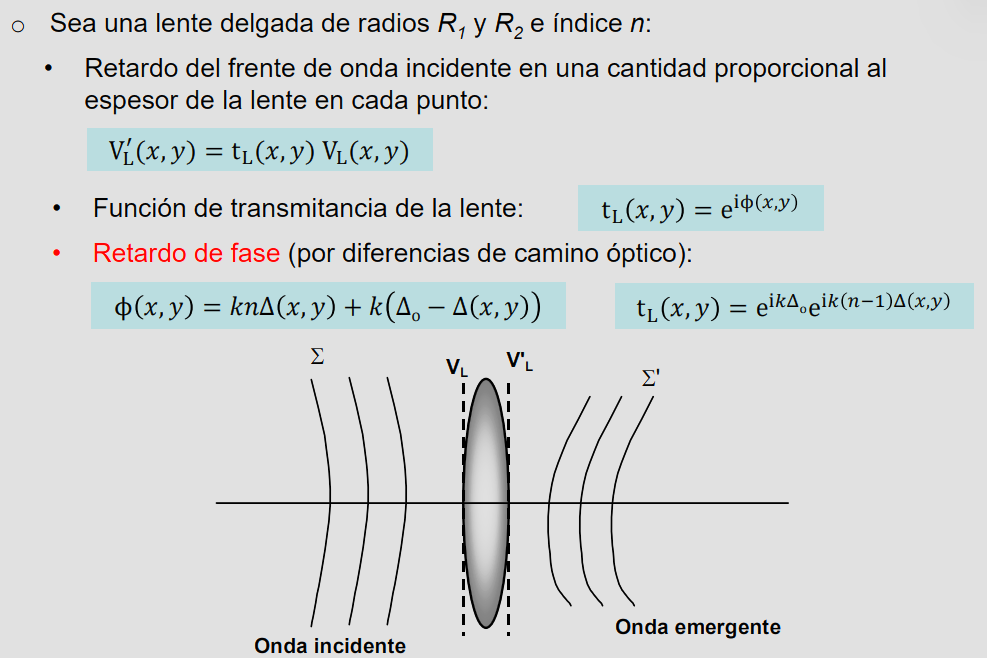
\includegraphics[width=0.7\textwidth]{IMG/lentdel.png}
	\end{figure}
	
	\esp
	
	El efecto de la lente delgada es retardar el frente de onda incidente en una cantidad proporcional al espesor de la lente en cada punto. De este modo, si $\Delta_o$ es el espesor máximo de la lente en el centro y $\Delta(x,y)$ el grosor de la lente en las coordenadas $(x,y)$. 
	
	\esp
	
	\noindent El retardo total de fase que sufre la onda al atravesar la lente viene dado por:
	
	\esp
	
	\begin{equation}
		\phi(x,y) = kn\Delta(x,y) + k(\Delta_o - \Delta(x,y))
	\end{equation}
	
	\esp
	
	donde $n$ es el índice de refracción del material de la lente, que supondremos perfectamente transparente y sumergida en aire. 
	
	\esp
	
	Por ello, podemos representar el comportamiento de la lente como una transformación de fase (función transmitancia) de la forma:
	
	\esp
	
	\begin{equation}
		t_L(x,y) = e^{i\phi(x,y)} = e^{ik\Delta_o}e^{ik(n-1)\delta(x,y)}
	\end{equation}
	
	\begin{figure}[H]
		\centering
		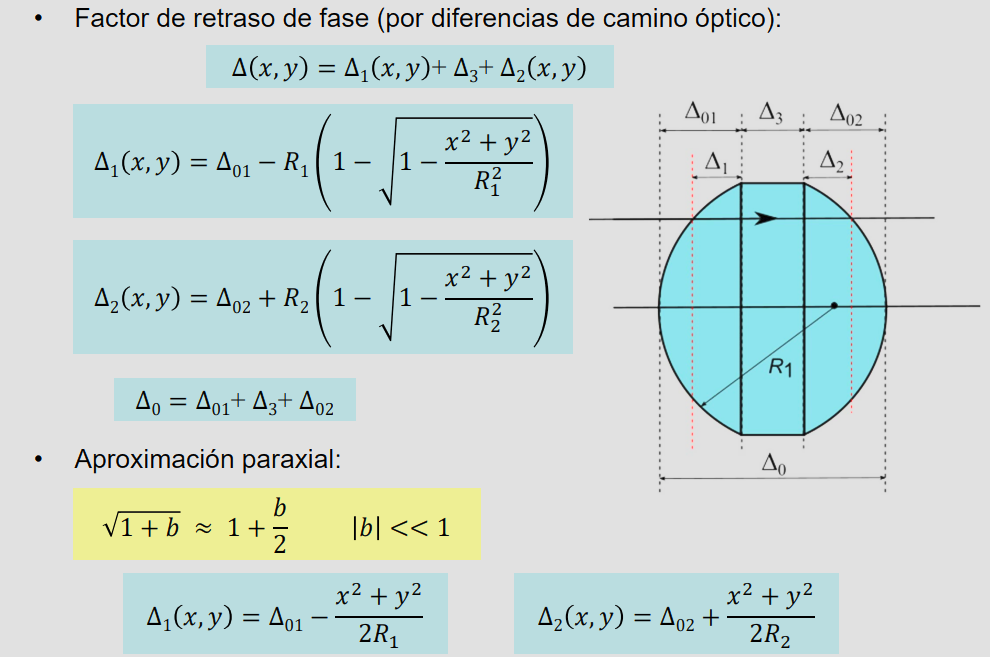
\includegraphics[width=0.7\textwidth]{IMG/lentdel2.png}
	\end{figure}
	
	\begin{figure}[H]
		\centering
		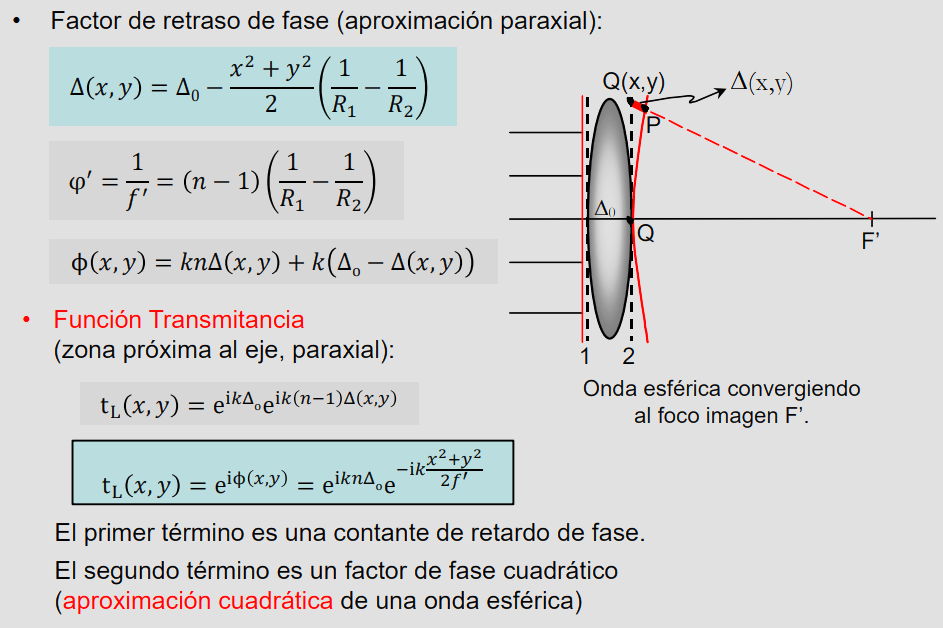
\includegraphics[width=0.7\textwidth]{IMG/lentdel3.png}
	\end{figure}
	

	
	\esp
	
	Si nos limitamos a considerar una región en torno al eje de la lente, entonces $\Delta(x,y) = (n-1)\delta(x,y) = (n-1)\Delta_o - f'(\sqrt{x^2+y^2} - 1)$, que en aproximación paraxial sería $\Delta(x,y) = \Delta_o - \frac{x^2+y^2}{2f'}$ una distribución de amplitud $V(x,y)$ a la entrada de la lente se convierte a su salida en:
	
	\esp
	
	\begin{equation}
		V'(x,y) = V(x,y)e^{ikn\Delta_o} e^{\frac{-ik}{2f'}(x^2+y^2)}
	\end{equation}
	
	\esp
	
	Aparte de un factor de fase constante, esta expresión se corresponde con lo que usualmente se denomina la aproximación cuadrática de una onda esférica, y nos indica que a la salida de la lente tendremos bien una onda convergente o divergente según sea $f' > 0$ ó $f' < 0$. Esta expresión puede obtenerse de forma alternativa utilizando los radios de curvatura de la lente y el recorrido en el interior del material de la misma, llegando al resultado anterior tras utilizar la aproximación paraxial y la expresión para la potencia de la lente delgada que se ha visto en Óptica Geométrica (Tema 1 de Óptica I):
	$\phi' = \frac{1}{f'} = (n-1) \left( \frac{1}{R_1} - \frac{1}{R_2} \right)$.
	
	\esp
	
	Comenzaremos el estudio de la formación de la imagen óptica evaluando la formación de la imagen de un objeto puntual (respuesta impulso), a partir de la cual, y por aplicación del principio de superposición, vamos a determinar y caracterizar la imagen de un objeto extenso.
	
	\subsection{Formación de imagen de un punto: PSF}
	
	\begin{figure}[H]
		\centering
		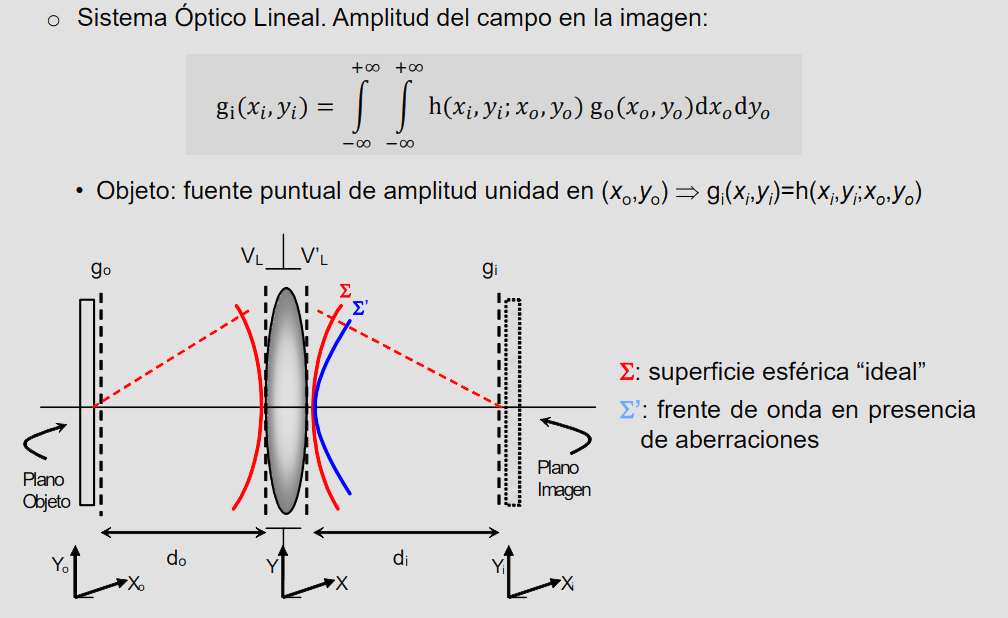
\includegraphics[width=0.7\textwidth]{IMG/psflente.png}
	\end{figure}

	\esp
	
	Abordamos ahora el tema más complejo de la formación de imagen cuando el haz de luz proviene del propio objeto, y se propaga difraccionalmente hacia la imagen. Basándonos en la linealidad de la propagación de las ondas podemos expresar la amplitud $V_i$ del campo en la imagen mediante la integral de superposición siguiente:

	\esp
	
	\begin{equation}
		V_i(x_i, y_i) = \int_{-\infty}^{+\infty} h(x_i, y_i; x_o, y_o) V_o(x_o, y_o) dx_o dy_o
	\end{equation}
	
	\esp
	
	donde $h(x_i, y_i; x_o, y_o)$ representa la respuesta impulso de la lente y $V_o(x_o, y_o)$ la amplitud del campo en el objeto.
	
	\esp
	
	\begin{figure}[H]
		\centering
		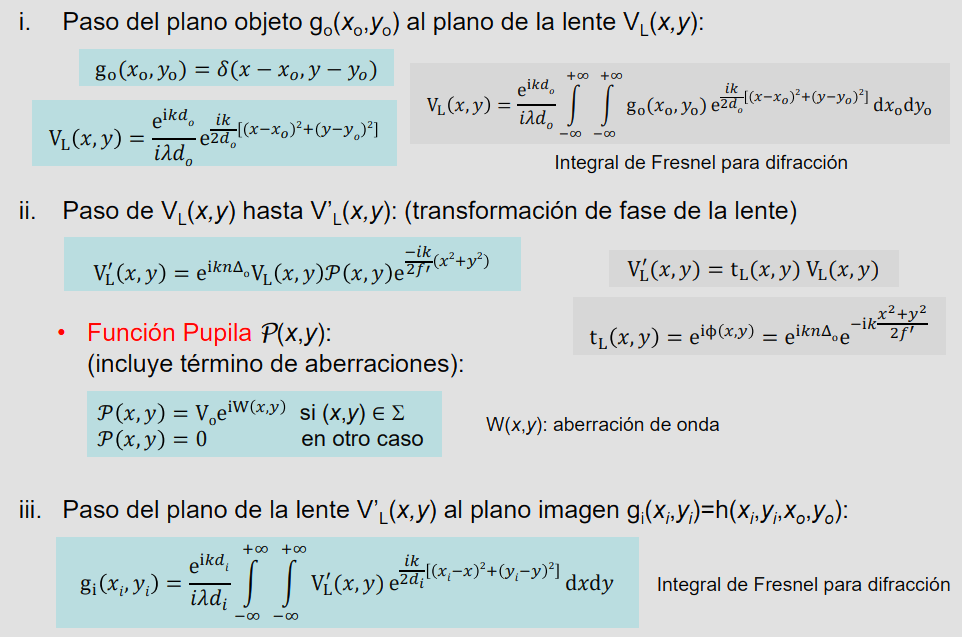
\includegraphics[width=0.7\textwidth]{IMG/psflente2.png}
	\end{figure}
	
	\esp
	
	La respuesta impulso habrá de evaluarse a partir del cálculo de la amplitud del campo obtenida en el punto $(x_i, y_i)$ del plano imagen, tomando como objeto una fuente puntual de amplitud unidad situada en el punto $(x_o, y_o)$ del plano objeto. De este modo, sobre la lente incidirá una onda esférica de amplitud unidad procedente del punto $(x_o, y_o)$, cuya amplitud puede calcularse a partir de la integral de Fresnel para la difracción, según la cual el campo en un punto $(x, y)$, justo delante de la lente a distancia $d_o$ del objeto, está dado por:
	
	\esp
	
	\begin{equation}
		V_L(x, y) = \frac{e^{ikd_o}}{i\lambda d_o} e^{\frac{ik}{2d_o} [(x-x_o)^2 + (y-y_o)^2]}
	\end{equation}
	
	\esp
	
	La amplitud del campo, $V'_L(x, y)$, en un plano justo detrás de la lente (teniendo en cuenta lo visto en la subsección anterior) vendrá dada por:
	
	\esp
	
	\begin{equation}
		V'_L(x, y) = V_L(x, y) \wp(x, y) e^{\frac{-ik}{2f'} (x^2 + y^2)}
	\end{equation}
	
	\esp
	
	donde se ha incluido la función $\wp(x, y)$ o función pupila, que tiene en cuenta la extensión finita de la lente y el hecho de que el frente de onda a la salida de la misma, si ésta es aberrante, no coincida con una superficie esférica ideal (figura 1). Esta función se puede expresar como:
	
	\esp
	
	\begin{equation}
		\wp(x, y) = \tau(x, y) e^{iW(x, y)}
	\end{equation}
	
	\esp
	
	siendo $\tau(x, y)$ constante si el sistema óptico tiene transmitancia uniforme, y $W(x, y)$ la aberración de onda. Si $W(x, y) = 0$ y $\tau(x, y) = 1$ se tratará de un sistema óptico perfecto.
	
	\esp
	
	\begin{figure}[H]
		\centering
		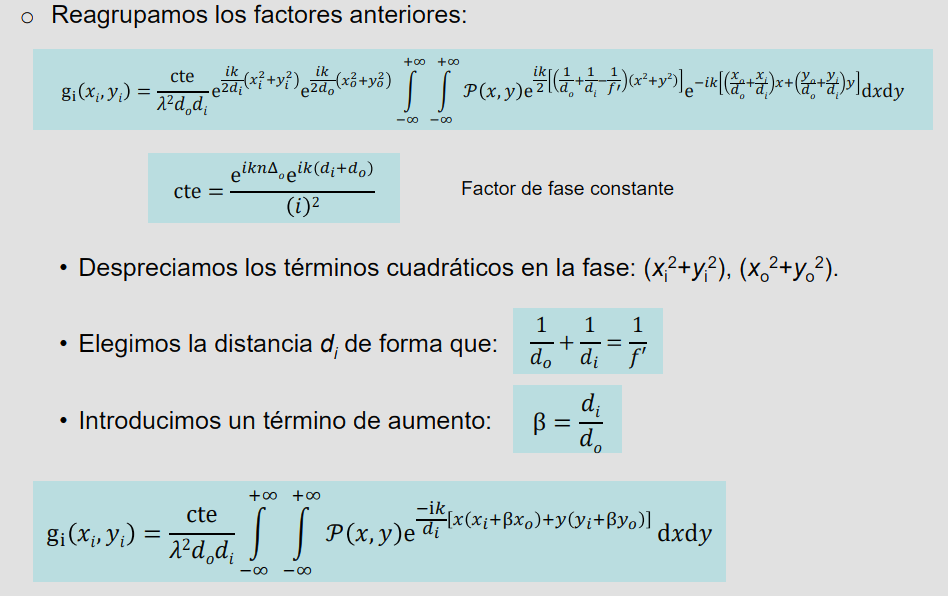
\includegraphics[width=0.7\textwidth]{IMG/psflente3.png}
	\end{figure}
	
	\esp
	
	En la figura 2, se ilustran los pasos necesarios para llegar desde el plano objeto hasta el plano imagen con nuestro planteamiento inicial.
	Finalmente, y después de propagarse una distancia $d_i$ y en el plano imagen (donde se verifica la ecuación de Gauss). 
	
	\esp
	
	\begin{figure}[H]
		\centering
		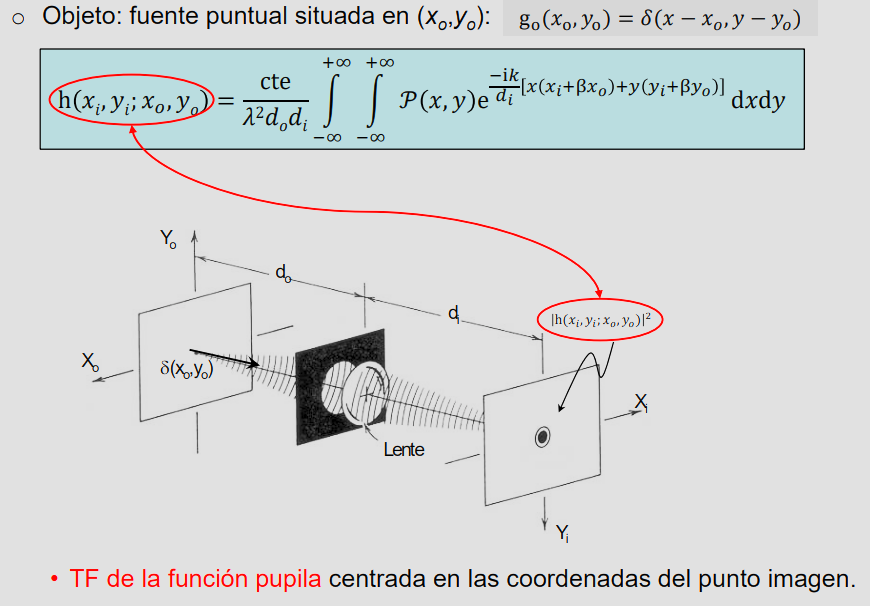
\includegraphics[width=0.7\textwidth]{IMG/psflente4.png}
	\end{figure}
	
	\esp
	
	La distribución de campo resultante $V_i(x_i, y_i)$ en dicho plano, que se identifica con la función respuesta impulso $h(x_i, y_i; x_o, y_o)$, quedará como:
	
	\esp
	
	\begin{equation}
		h(x_i, y_i; x_o, y_o) = \frac{1}{\lambda^2 d_i d_o} \iint_{-\infty}^{+\infty} \wp(x, y) e^{\frac{-ik}{d_i} [(x_i + \beta x_o)x + (y_i + \beta y_o)y]} dx dy
	\end{equation}
	
	\esp
	
	donde se han omitido los factores de fase constantes, y se ha considerado despreciable la contribución de los factores de fase cuadráticos... El coeficiente que se ha introducido ($\beta = \frac{d_i}{d_o}$), sería el aumento lateral del sistema. Por tanto, una fuente puntual objeto produce una distribución en amplitud en el espacio imagen que viene dada, salvo por un factor de escala, por el modelo de difracción de Fraunhöfer de la función pupila de la lente, con el patrón de difracción centrado en las coordenadas imagen ($x_i = -\beta x_o, y_i = -\beta y_o$).
	
	\subsubsection{Formación de la imagen}
	
	\begin{figure}[H]
		\centering
		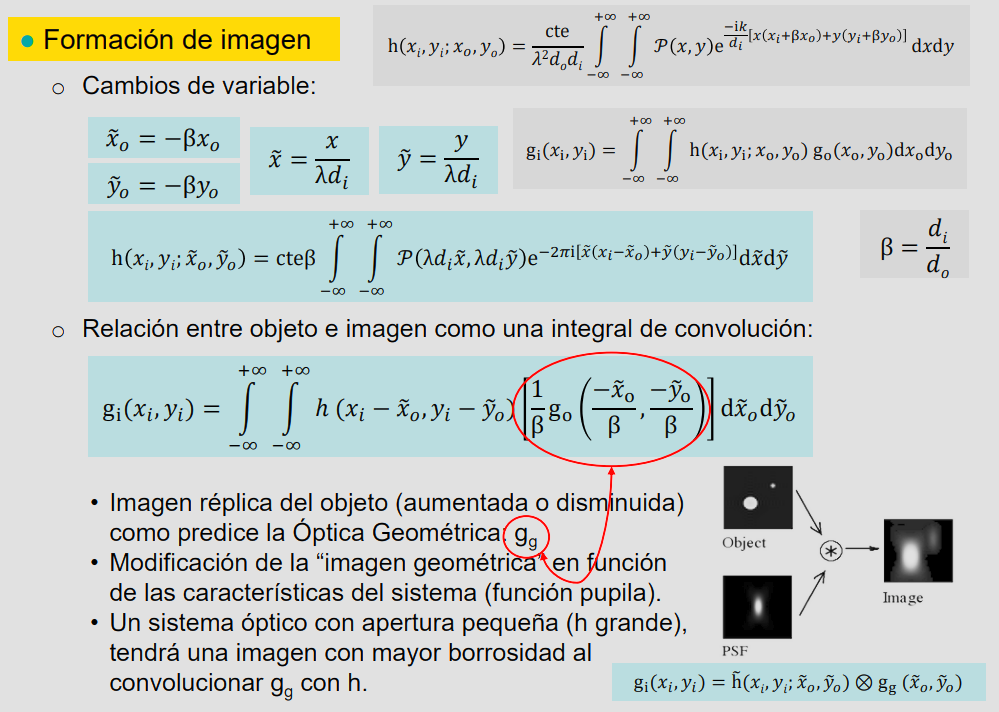
\includegraphics[width=0.7\textwidth]{IMG/psflente5.png}
	\end{figure}
	
	\esp
	
	Con el fin de reducir la relación objeto-imagen a una expresión matemática que sea conocida, como es la integral de convolución, hagamos los siguientes cambios de variables para las coordenadas objeto que aparecen en la ecuación anterior:
	
	\esp
	
	\begin{align}
		\tilde{x}_o &= -\beta x_o \\
		\tilde{y}_o &= -\beta y_o \\
		\tilde{x} &= \frac{x}{\lambda d_i} \\
		\tilde{y} &= \frac{y}{\lambda d_i}
	\end{align}
	
	\esp
	
	\noindent Obtenemos entonces para la respuesta impulso:
	
	\esp
	
	\begin{equation}
		h(x_i, y_i; \tilde{x}_o, \tilde{y}_o) = \beta \iint_{-\infty}^{+\infty} \wp(\lambda d_i \tilde{x}, \lambda d_i \tilde{y}) e^{-2\pi i [(x_i - \tilde{x}_o)\tilde{x} + (y_i - \tilde{y}_o)\tilde{y}]} d\tilde{x}d\tilde{y}
	\end{equation}
	
	\esp
	
	De este modo, si definimos $\tilde{h} = \frac{h}{\beta}$, la integral de superposición para la formación de imagen resulta ser la convolución de la respuesta impulso con la imagen $V_g$, que sería una transformación del objeto considerando sólo propiedades geométricas:
	
	\esp
	
	\begin{equation}
		V_i(x_i, y_i) = \iint_{-\infty}^{+\infty} \tilde{h}(x_i - \tilde{x}_o, y_i - \tilde{y}_o) \frac{1}{\beta} V_o \left( \frac{-\tilde{x}_o}{\beta}, \frac{-\tilde{y}_o}{\beta} \right) d\tilde{x}_o d\tilde{y}_o
	\end{equation}
	
	\esp
	
	\begin{equation}
		V_i(x_i, y_i) = \tilde{h}(x_i, y_i) \otimes V_g(x_i, y_i)
	\end{equation}
	
	\esp
	
	donde $V_g(x_i, y_i) = \frac{1}{\beta} V_o \left( \frac{-x_i}{\beta}, \frac{-y_i}{\beta} \right)$. Por tanto, cuando se introduzcan los efectos de la difracción, la imagen dejará de ser una réplica exacta del objeto como consecuencia del ancho de banda no nulo de la respuesta impulso del sistema. Esto provocará que se atenúen los detalles del objeto con la correspondiente pérdida de fidelidad entre éste y su imagen.

	\printbibliography[title={Bibliografía}]
\end{document}